
\chapter{Background} % Main chapter title

\label{Background} % For referencing the chapter elsewhere, use \ref{Background} 

\lhead{Chapter \ref{Background}. \emph{Background}} % This is for the header on each page - perhaps a shortened title

The background of this thesis is concerned with the algorithms related to our work and how they were accelerated by many studies on CUDA-enabled GPUs.

%----------------------------------------------------------------------------------------

\section{Sequence alignment and protein database}
\subsection{Cells, amino acids and proteins}

In 1665, Robert Hooke discovered the cell \citep{Cell}. The cell theory, first developed in 1839 by Matthias Jakob Schleiden and Theodor Schwann, generalized the view that \emph{all living organisms are composed of cells and of cell products} \citep{Loewy}. As workhorses of the cell, proteins not only constitute the major component in the cell, but they also regulate almost all activities that occurs in living cells.

Proteins are complex chains of small organic molecules known as \emph{amino acids}. In this thesis, \emph{residue} is used to refer to amino acids for protein. The 20 amino acids detailed in Table \ref{tab.amino} have been found within proteins and they convey a vast array of chemical versatility. So proteins can be viewed as sequences of an alphabet of the 20 amino acids \{A,C,D,E,F,G,H,I,K,L,M,N,P,Q,R,S,T,V,W,Y\}.

\begin{table}[H]
\centering
\begin{tabular}{|c|c|c|c|}\hline
\textbf{Letter} & \textbf{Amino acid} & \textbf{Letter} & \textbf{Amino acid} \\\hline
A & Alanine & C & Cysteine \\\hline
D & Aspartic acid & E & Glutamic acid \\\hline
F & Phenylalanine & G & Glycine \\\hline
H & Histidine & I & Isoleucine \\\hline
K & Lysine & L & Leucine \\\hline
M & Methionine & N & Asparagine \\\hline
P & Proline & Q & Glutamine \\\hline
R & Arginine & S & Serine  \\\hline
T & Threonine & V & Valine   \\\hline
W & Tryptophan & Y & Tyrosine  \\\hline
\end{tabular}
\caption{\fontfamily{pag}\selectfont The 20 amino acids\label{tab.amino}}
\end{table}

The following is the protein sequence of human beta globin taken from Swiss-Prot database. The sequence has a entry name HBB\_HUMAN in Swiss-Prot database. The number beside the residue indicates the position of the residue.

\begin{verbatim}
   HBB_HUMAN   1 MVHLTPEEKS AVTALWGKVN VDEVGGEALG RLLVVYPWTQ RFFESFGDLS 50
   HBB_HUMAN  51 TPDAVMGNPK VKAHGKKVLG AFSDGLAHLD NLKGTFATLS ELHCDKLHVD 100 
   HBB_HUMAN 101 PENFRLLGNV LVCVLAHHFG KEFTPPVQAA YQKVVAGVAN ALAHKYH 147
\end{verbatim}

\subsection{Sequence alignment}
In bioinformatics, a sequence alignment is a way of arranging the sequences of protein to identify regions of similarity \citep{sa}. If two amino acid sequences are recognized as similar, there is a chance that they are \emph{homologous}. Homologous sequences share a common functional, structural, or evolutionary relationships between them. Protein sequences evolve by accumulating mutations. The basic mutational process are \emph{substitutions} where one residue is replaced by another, \emph{insertions} where a new residue is inserted into the sequence, and \emph{deletions}, the removal of a residue. Insertions and deletions are together referred to as \emph{gaps}. Table \ref{tab.sa} shows the sequence alignment of human beta globin (the \emph{query} sequence) and myoglobin (the \emph{target} sequence) and an internal gap is indicated by two dashes \citep{BioFunc}.

In the pairwise alignment shown in .., globins4 is on top and HBB\_HUMAN is below. Note that this particular alignment is called \emph{local} because only a subset of the two proteins is aligned: the first residue of HBB\_HUMAN is not displayed. A global pairwise alignment includes all residues of both sequences. An intermediate row indicates the presence of \emph{identical} residues in the alignment. Some of the aligned residues are similar but not identical; they are related to each other because they share similar biochemical properties. \emph{Similar} pairs of residues are structurally or functionally related. For example, on the first part of the alignment we can find V and H connected by a + sign; nearby we can see S and T aligned. These are \emph{conservative substitutions}.

\begin{verbatim}
    globins4   1 VVLSEAEKTKVKAVWAKVEADVEESGADILVRLFKSTPATQEFFEKFKDL 50
                 V+L+++EK++V+A+W+KV  +V+E+G+++L RL++++P+TQ+FFE+F+DL
   HBB_HUMAN   2 VHLTPEEKSAVTALWGKV--NVDEVGGEALGRLLVVYPWTQRFFESFGDL 49
  
    globins4  51 STEDELKKSADVKKHGKKVLDALSDALAKLDEKLEAKLKDLSELHAKKLK 100 
                 ST+D+++++++VK+HGKKVL+A+SD+LA+LD +L++++++LSELH++KL+
   HBB_HUMAN  50 STPDAVMGNPKVKAHGKKVLGAFSDGLAHLD-NLKGTFATLSELHCDKLH 98 

    globins4 101 VDPKYFKLLSEVLVDVLAARLPKEFTADVQAALEKLLALVAKLLASKYK 149
                 VDP++F+LL++VLV+VLA++++KEFT++VQAA++K++A VA++LA+KY+
   HBB_HUMAN  99 VDPENFRLLGNVLVCVLAHHFGKEFTPPVQAAYQKVVAGVANALAHKYH 147
\end{verbatim}


\begin{table}[H]
\centering
\begin{tabular}{|c|c|c|c|c|}\hline
\textbf{Query} & V T A L W & G K V N V & D -\hspace{6pt}-\hspace{6pt}E V & G G E A L \\\hline
\textbf{Target} & V L N V W & G K V E A & D I P G H & G Q E V L \\\hline
\emph{match} & 4\hspace{36pt} 11 & 6\hspace{8pt}5\hspace{8pt}4\hspace{19pt} & 6\hspace{44pt} & 6\hspace{18pt}5\hspace{18pt}4 \\\hline
\emph{mismatch} &-1-2 1 & \hspace{40pt}0\hspace{7pt}0 & \hspace{28pt}-2 -3 & -2\hspace{15pt} 0 \\\hline
\shortstack{\emph{gap open}\\ \emph{gap extend}} & & & \shortstack{-11\hspace{26pt} \\ -1} & \\\hline
\end{tabular}
\caption{\fontfamily{pag}\selectfont \textbf{Sequence alignment} \\sum of \emph{match}: +51\\sum of \emph{mismatch}: -9\\sum of gap penalties: -12\\total raw score: 51 - 9 -12 = 30\label{tab.sa}}
\end{table}

To establish the degree of similarity, the two sequences are aligned: lined up in such a way that the similarity score is maximized. Table \ref{tab.sa} illustrates how raw scores are calculated. The scores in the table for \emph{match/mismatch} are taken from the scoring matrix BLOSUM62 as shown in Figure \ref{fig:blo}. The BLOSUM62 matrix is a substitution matrix used for sequence alignment of proteins. It were first introduced in a paper by S. Henikoff and J.G. Henikoff \citep{Henikoff}. In a typical scoring scheme there are two gap penalties: one for \emph{gap open} (-11 in the example of Table \ref{tab.sa}) and one for \emph{gap extend} (-1 in Table \ref{tab.sa}).

\begin{figure}[!htb]
\centering
	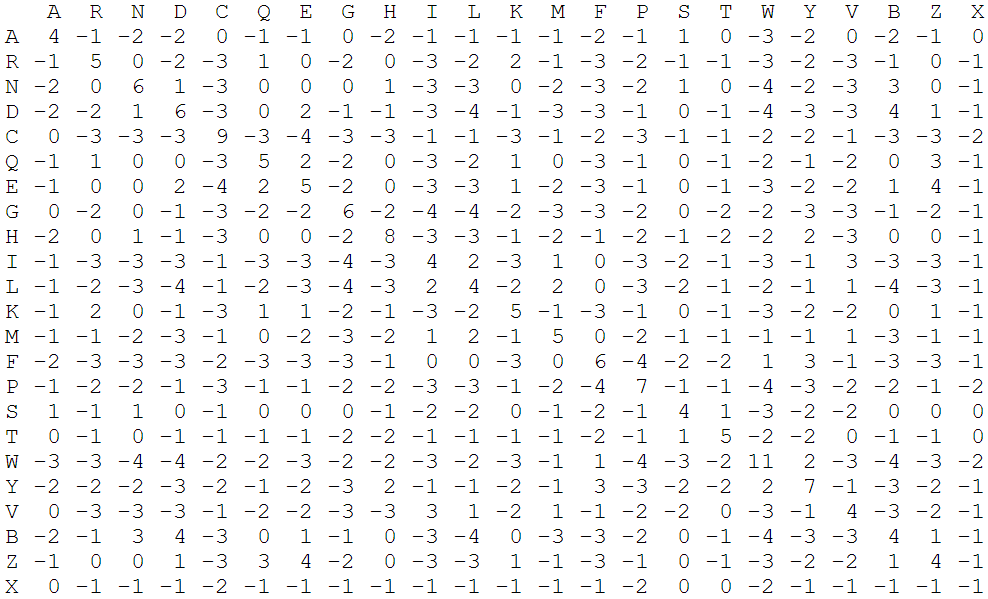
\includegraphics[width=140mm]{Figures/BLOSUM62.png}
	\caption{\fontfamily{pag}\selectfont BLOSUM62 Scoring Matrix from \url{http://www.ncbi.nlm.nih.gov/Class/FieldGuide/BLOSUM62.txt}.}
	\label{fig:blo}
\end{figure}

Next chapter will introduce two sequence alignment algorithms: Smith-Waterman algorithm and HMM-based algorithm. These two algorithms share a very general optimization technique called dynamic programming for finding optimal alignments.

\subsection{Bioinformatics protein databases}
This part is a brief introduction of two protein sequence databases used in this thesis.

\subsubsection*{NCBI NR databse}
The NCBI (National Center for Biotechnology Information) houses a series of databases relevant to Bioinformatics. Major databases include GenBank for DNA sequences and PubMed, a bibliographic database for the biomedical literature. Other databases include the NCBI Epigenomics database. All these databases are updated daily and available online: \url{http://www.ncbi.nlm.nih.gov/guide/all/\#databases\_}.

The NR (Non-Redundant) protein database maintained by NCBI as a target for their BLAST search services is a composite of Swiss-Prot, Swiss-Prot updates, PIR(Protein Information Resource), PDB(Protein Data Bank). Entries with absolutely identical sequences have been merged into NR database. The PIR produces the largest, most comprehensive, annotated protein sequence database in the public domain. The PDB is a repository for the three-dimensional structural data of large biological molecules, such as proteins and nucleic acids and is maintained by Brookhaven National Laboratory, USA.

Release 2014\_04 of NCBI NR databse contains 38,442,706 sequence entries, comprising 13,679,143,700 amino acids, more than 24GB in file size \citep{NCBI}.

\subsubsection*{Swiss-Prot}
The Universal Protein Resource (UniProt) is a comprehensive resource for protein sequence and annotation data and is mainly supported by the National Institutes of Health (NIH) \citep{upr}. The UniProt databases are the UniProt Knowledgebase (UniProtKB), the UniProt Reference Clusters (UniRef), and the UniProt Archive (UniParc). 

The UniProt Knowledgebase is updated every four weeks on average and consists of two sections: 
\begin{itemize}
 \item UniProtKB/Swiss-Prot\\
 This section contains manually-annotated records with information extracted from literature and curator-evaluated computational analysis. It is also highly cross-referenced to other databases. Release 2014\_05 of 14-May-2014 of UniProtKB/Swiss-Prot contains 545,388 sequence entries, comprising 193,948,795 amino acids abstracted from 228,536 references \citep{Swiss-Prot}.
 \item UniProtKB/TrEMBL\\
 This section contains computationally analyzed records that await full manual annotation. Release 2014\_05 of 14-May-2014 of UniProtKB/TrEMBL contains 56,010,222 sequence entries, comprising 17,785,675,050 amino acids \citep{UniProtTr}.
\end{itemize}

%----------------------------------------------------------------------------------------

\section{Dynamic programming in Bioinformatics}
Dynamic Programming (DP) is an optimization technique that recursively breaks down a problem into smaller subproblems, such that the solution to the larger problem can be obtained by piecing together the solutions to the subproblems \citep{BioMach}. This section shows how the Smith-Waterman algorithms and the algorithms in HMMER use DP for sequence alignment and database searches, and then discusses the related work about acceleration on CUDA-enabled GPU.

\subsection{The Smith-Waterman algorithm}
The Smith-Waterman algorithm is designed to find the optimal local alignment between two sequences. It was proposed by Smith and Waterman \citep{SW} and enhanced by Gotoh \citep{Gotoh}. The alignment of two sequences is based on dynamic programming approach by computing the similarity score which is given in the form of similarity score matrix $H$. 

Given a query sequence $Q$ with length $L_q$ and a target sequence $T$ with length $L_t$, let $S$ be the substitution matrix and its element $S[i,j]$ be the similarity score for the combination of the $i^{th}$ residue in $Q$ and the $j^{th}$ residue in $T$. Define $G_e$ as the gap extension penalty, and $G_o$ as the gap opening penalty. These similarity scores and $G_e$, $G_o$ are pre-determined by the life sciences community. The similarity score matrix $H$ for aligning $Q$ and $T$ is calculated as 

\begin{equation*}
   E[i, j] = max 
   \begin{cases}
    E[i, j-1]-G_e\\
    H[i, j-1]-G_o
   \end{cases}
\end{equation*}
\begin{equation*}
   F[i, j] = max
   \begin{cases}
    F[i-1, j]-G_e\\
    H[i-1, j]-G_o
   \end{cases}
\end{equation*}
\begin{equation*}
   H[i, j] = max
   \begin{cases}
    0\\
    E[i, j]\\
    F[i,j]\\
    H[i-1, j-1] + S[i,j]
   \end{cases}
\end{equation*}

where $1\leqslant i \leqslant L_q$ and $1\leqslant j \leqslant L_t$. The values for $E$, $F$ and $H$ are initialized as $E[i,0] = F[0,j] = H[i,0] = H[0,j]$ when $0\leqslant i \leqslant L_q$ and $0\leqslant j \leqslant L_t$.

The maximum value of the matrix $H$ gives the similarity score between $Q$ and $T$.

%----------------------------------------------------------------------------------------
\subsection{HMMER}

\label{HMMERsect}

HMMER \citep{HMMER} is a set of applications that create a profile Hidden Markov Model (HMM) of a sequence family which can be utilized as a query against a sequence database to identify (and/or align) additional homologs of the sequence family\citep{Seq}. HMMER was developed by Sean Eddy at Washington University and has become one of the most widely used software tools for sequence homology. The main elements of this HMM-based sequence alignment package are \emph{hmmsearch} and \emph{hmmscan}. The former searches a profile HMM against a sequence database, while the latter searches a sequence against a profile HMMs database.

\subsubsection{HMM and profile HMM}

A hidden Markov model (HMM) is a computational structure for linearly analyzing sequences with a probabilistic method \citep{DicBioinfo}. HMMs have been widely used in speech signal, handwriting and gesture detection problems. In bioinformatics they have been used for applications such as sequence alignment, prediction of protein structure, analysis of chromosomal copy number changes, and gene-finding algorithm, etc \citep{BioFunc}. 

A HMM is a type of a non-deterministic finite state machine with transiting to another state and emitting a symbol under a probabilistic model.
According to \citep{SeqData}, a HMM can be defined as a 6-tuple ($A$, $Q$, $q_0$, $q_e$, $tr$, $e$) where \\[-1cm]

\begin{itemize}
\item \textbf{$A$} is a finite set (the alphabet) of symbols;
\item \textbf{$Q$} is a finite set of \emph{states};
\item \textbf{$q_0$} is the \emph{start} state and \textbf{$q_e$} is the \emph{end} state;
\item \textbf{$tr$} is the \emph{transition} mapping, which is the transition probabilities of state pairs in $Q$ $\times$ $Q$, satisfying the following two conditions: 
  \begin{enumerate}
   \item[(a)] $0 \leqslant tr(q,q') \leqslant 1$, $\forall q,q' \in Q$, and
   \item[(b)] for any given state $q$, such that:
   \begin{equation*}
    \displaystyle\sum_{q' \in Q}tr(q,q') = 1
   \end{equation*}
  \end{enumerate}
\item \textbf{$e$} is the \emph{emission} mapping, which is the emission probabilities of pairs in $Q$ $\times$ $A$, satisfying the following two conditions:
  \begin{enumerate}
   \item[(a)] $0 \leqslant e(q,x) \leqslant 1$, if it is defined, $\forall q \in Q$, and $x \in A$
   \item[(b)] for any given state $q$, if for any $x \in A$, $e(q, x)$ is defined, then $q$ is an \emph{emitting} state and
   \begin{equation*}
    \displaystyle\sum_{x \in A}e(q,x) = 1 
   \end{equation*}
   if $\forall x \in A$, $e(q, x)$ is not defined, then $q$ is a \emph{silent} state.
  \end{enumerate}
\end{itemize}

The dynamics of the system is based on Markov Chain, meaning that only the current state influences the selection of its successor – the system has no `memory' of its history. Only the succession of characters emitted is visible; the state sequence that generated the characters remains internal to the system, i.e. hidden. By this means, the name is Hidden Markov Model\citep{IntroBio}. 

Profile HMM is a variant of HMM and can be constructed from an initial multiple sequence alignment to define a set of probabilities. The symbol sequence of an HMM is an observed sequence that resembles a consensus for the multiple sequence alignment. And a protein family can be defined by profile HMMs.

In Figure \ref{fig:pHMM}, the internal structure of the ``Plan 7" profile HMM used by HMMER\citep{HMMER3} shows the mechanism for generating sequences. In order to generate sequences, a profile HMM should have a set of three states per alignment column: one \emph{match} state, one \emph{insert} state and one \emph{delete} state. 
\begin{itemize}
\item \textbf{\emph{match state}} matches and emits a amino acid from the query. The probability of emitting each of the 20 amino acids is a property of the model. 
\item \textbf{\emph{insert state}} allows the insert of one or more amino acids. The emission probability of this state is computed either from a background distribution of amino acids or from the observed insertions in the alignment.
\item \textbf{\emph{delete state}} skips the alignment column and emits a blank. Entering this state corresponds to gap opening, and the probabilities of these transitions reflect a position-specific gap penalty.
\end{itemize}

\begin{figure}[!htb]
	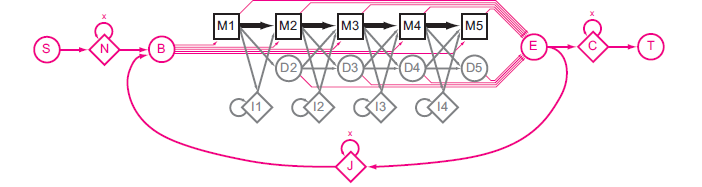
\includegraphics[width=150mm]{Figures/pHMM.png}
	\caption{\fontfamily{pag}\selectfont Profile HMM architecture used by HMMER\citep{HMMER3}.}
	\label{fig:pHMM}
\end{figure}

The structure begins at Start(S), and follows some chain of arrows until arriving at Termination(T). Each arrow transits to a state of the system. 
At each state, an action can be taken either as (1) emitting a residue, or (2) selecting an arrow to the next state. The action and the selection of successor state are governed by sets of probabilities\citep{IntroBio}.
The linear core model has five sets of match (M), insert (I) and delete (D) states. Each M state represents one consensus position and a set of M, I, D states is the main element of the model and is referred to as a ``node''� in HMMER. Additional flanking states (marked as N, C, and J) emit zero or more residues from the background distribution, modelling nonhomologous regions preceding, following, or joining homologous regions aligned to the core model. Start (S), begin (B), end (E) and termination (T) states are non-emitting states.

A profile HMM for a protein family can be used to compare with target sequences, and classify sequences that are members of the family and those which are not\citep{ProteinBio}. 
A common application of profile HMMs is used to search a profile HMM against a sequence database. Another application is the query of a single protein sequence of interest against a database of profile HMMs.

\subsubsection{Viterbi algorithm in HMMER2}

\label{ViterbiSub}

In HMMER2, both \emph{hmmsearch} and \emph{hmmpfam} rely on the same core Viterbi algorithm for their scoring function which is named as \emph{P7Viterbi} in codes.

To find whether a sequence is member of the family described by a HMM, we compare the sequence with the HMM. We use an algorithm known as Viterbi to find one path that has the maximum probability of the HMM generating the sequence. Viterbi is a dynamic programming algorithm. Let $V_{i,j}$ be the maximum probability of a path from the start state $S_i$ ending at state $S_j$ and generating the prefix $q_{1...j}$ of the target sequence. $V_{i+1,j}$ is found by the recurrence:

\begin{equation*}
   \displaystyle V_{i+1,j} = \max_{0 \leqslant k \leqslant j-1} \big ( V_{i,k} P(k,j)P(q_{i+1} |j) \big )
\end{equation*}

% max |x| = 
%     \begin{cases}
%     \quad -x & \text{if } x < 0,\\
%     0 & \text{if } x = 0,\\
%     x & \text{if } x > 0.
%     \end{cases}
%     max = \left\{
% \begin{array}{rl}
% -x & \text{if } x < 0,\\
% 0 & \text{if } x = 0,\\
% x & \text{if } x > 0.
% \end{array} \right.

Define $a[i,j]$ as the transition probability from state $i$ to $j$ and $e_i$ as emission probability in state $i$.
Define $V_j^M(i)$ as the log-odds score of the optimal path matching subsequence $x_{1...i}$ to the submodel up to state $j$, ending with $x_i$ being emitted by \emph{match} state $M_j$. Similarly $V_j^I(i)$ is the score of the optimal path ending in $x_i$ being emitted by \emph{insert} state $I_j$, and $V_j^D(i)$ for the optimal path ending in \emph{delete} state $D_j$. $q_{x_i}$ is the probability of $x_i$. Then we can write the Viterbi general equation\citep{BioSeq}:

\begin{equation*}
   V_j^M(i) = \log\frac{e_{M_j}(x_i)}{q_{x_i}} + max 
   \begin{cases}
   V_{j-1}^M(i-1) + \log a[M_{j-1},M_j]\\
   V_{j-1}^I(i-1) + \log a[I_{j-1},M_j]\\
   V_{j-1}^D(i-1) + \log a[D_{j-1},M_j]
   \end{cases}
\end{equation*}

\begin{equation*}
   V_j^I(i) = \log\frac{e_{I_j}(x_i)}{q_{x_i}} + max 
   \begin{cases}
   V_j^M(i-1) + \log a[M_j,I_j]\\
   V_j^I(i-1) + \log a[I_j,I_j]
   \end{cases} 
\end{equation*}

\begin{equation*}
   V_j^D(i) = max 
   \begin{cases}
   V_{j-1}^M(i) + \log a[M_{j-1},D_j]\\
   V_{j-1}^D(i) + \log a[D_{j-1},D_j]
   \end{cases}  
\end{equation*}

Based on the above equations, we can write the efficient pseudo code of Viterbi algorithm, as shown in Algorithm \ref{Viterbi} \citep{FPGA}.  The inner loop of the code contains three two dimensional matrices (M, I, D), which calculate scores of all node positions involved in the main models for each of the residue. The outer loop consists of flanking and special states calculated in the one dimensional arrays N, B, C, J, E.

\renewcommand{\thepseudonum}{\roman{pseudonum}}
\begin{pseudocode}{Viterbi}{ }
\label{Viterbi}
\COMMENT{Initialization}\\
N[0] \GETS 0; \ \  B[0] \GETS tr(N, B)\\
E[0] \GETS C[0] \GETS J[0] \GETS -\infty\\
\COMMENT{for every sequence residue i}\\
\FOR i \GETS 1 \TO L_t \DO
\BEGIN
  N[i] \GETS N[i-1] + tr(N, N)\\
  B[i] \GETS max 
  \begin{cases}
   N[i-1] + tr(N, B)\\
   J[i-1] + tr(J, B)
  \end{cases}\\
  M[i,0] \GETS I[i,0] \GETS D[i,0] \GETS -\infty\\
  \COMMENT{For every model position j from 1 to $L_q$}\\
  \FOR j \GETS 1 \TO L_q \DO
  \BEGIN
    M[0, j] \GETS I[0, j] \GETS D[0, j] \GETS -\infty\\
    M[i, j] \GETS e(M_j, S[i]) + max 
    \begin{cases}
     M[i-1, j-1] + tr(M_{j-1}, M_j)\\
     I[i-1, j-1] + tr(I_{j-1}, M_j)\\
     D[i-1, j-1] + tr(D_{j-1}, M_j)\\
     B[i-1] + tr(B, M_j)
    \end{cases}\\
    I[i, j] \GETS e(I_j, S[i]) + max
    \begin{cases}
     M[i-1, j] + tr(M_j, I_j)\\
     I[i-1, j] + tr(I_j, I_j)
    \end{cases}\\
    D[i, j] \GETS max
    \begin{cases}
     M[i, j-1] + tr(M_{j-1}, D_j)\\
     D[i, j-1] + tr(D_{j-1}, D_j)
    \end{cases}\\
  \END\\
  E[i] \GETS max\{M[i,j] + tr(M_j, E)\} \ \  (j \GETS 0 \TO L_q)\\
  J[i] \GETS max 
  \begin{cases}
   J[i-1] + tr(J, J)\\
   E[i-1] + tr(E, J)
  \end{cases}\\
  C[i] \GETS max
  \begin{cases}
   C[i-1] + tr(C, C)\\
   E[i-1] + tr(E, C)
  \end{cases}\\
\END\\
\COMMENT{Termination: }\\
\RETURN {T(S,M) \GETS C[L_t] + tr(C,T)}
\end{pseudocode}

From Algorithm \ref{Viterbi}, we can see the fundamental task of the Viterbi algorithm for biological sequence alignment is to calculate three DP(Dynamic Programming) matrices: $M[{ }]$ for Match state, $I[{ }]$ for Insert state and $D[{ }]$ for Delete state. Each DP matrix consisting of $(L_t+1) * (L_q+1)$ blocks, where each value of block is dependent on the value of previous block. As shown in Figure \ref{fig:dpV}, the Match state $M[i,j]$ depends on the upper-left block $M[i-1, j-1]$, $I[i-1, j-1]$ and $D[i-1, j-1]$; the Insert state $I[i,j]$ depends on the left block $M[i-1, j]$ and $I[i-1, j]$; and the Delete state depends on the upper block $M[i, j-1]$ and $D[i, j-1]$.

\begin{figure}[!htb]
\centering
	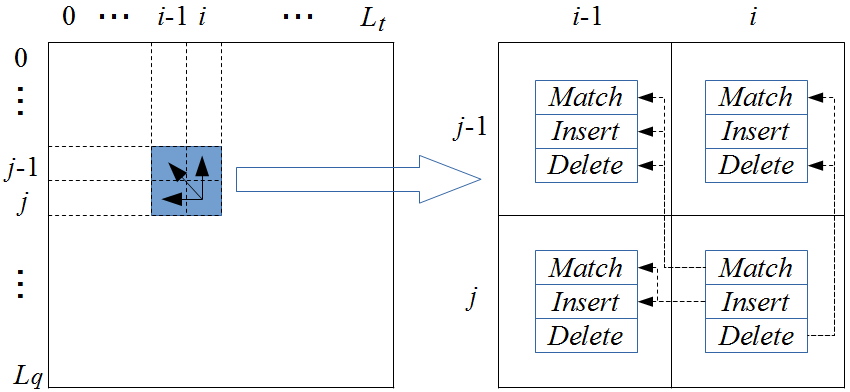
\includegraphics[width=120mm]{Figures/dpViterbi.png}
	\caption{\fontfamily{pag}\selectfont \textbf{The DP matrix calculated in Viterbi algorithm.} 
The rectangle on the left represents the whole matrix to be calculated by the Viterbi algorithm, and the right rectangle of the figure shows the process of updating a single block of the matrix.}
	\label{fig:dpV}
\end{figure}

\subsubsection{MSV algorithm in HMMER3}

\label{MSVsub}

HMMER3 is near rewrite of the earlier HMMER2 package, with the aim of improving the speed of profile HMM searches. The main performance gain is due to a heuristic algorithm called MSV filter, for Multiple (local, ungapped) Segment Viterbi. MSV is implemented in SIMD(Single-Instruction Multiple-Data) vector parallelization instructions and is about 100-fold faster than HMMER2.

\begin{figure}[!htb]
	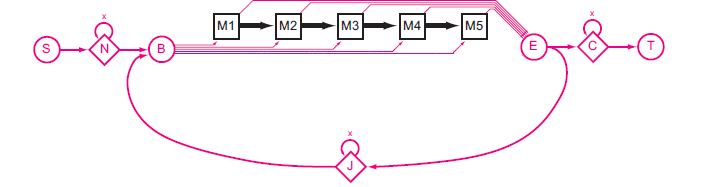
\includegraphics[width=150mm]{Figures/pHMM_msv.png}
	\caption{\fontfamily{pag}\selectfont MSV profile: multiple ungapped local alignment segments \citep{HMMER3}.}
	\label{fig:pMSV}
\end{figure}

Figure \ref{fig:pMSV} illustrates the MSV profile architecture. Compared with Figure \ref{fig:pHMM}, the MSV corresponds to the virtual removal of the delete and insert states. All match-match transition probabilities are treated as 1.0. The rest parameters remains unchanged. So this model generates sequences containing one or more ungapped local alignment segments. The pseudo code of MSV score algorithm is simplified and shown in Algorithm \ref{MSV}.

Figure \ref{fig:dpMSV} illustrates an example of an alignment of a MSV profile HMM model (length $L_q = 14$) to a target sequence (length $L_t=22$). A path to generate the target sequence with the profile HMM model is shown through a dynamic programming (DP) matrix. The model identifies two high-scoring ungapped alignment segments, as shown in black dots, indicating residues aligned to profile match states. All other residues are assigned to N, J, and C states in the model, as shown in orange dots. Unfilled dot indicates a ``mute'' non-emitting state or state transition.

\begin{figure}[!htb]
\centering
	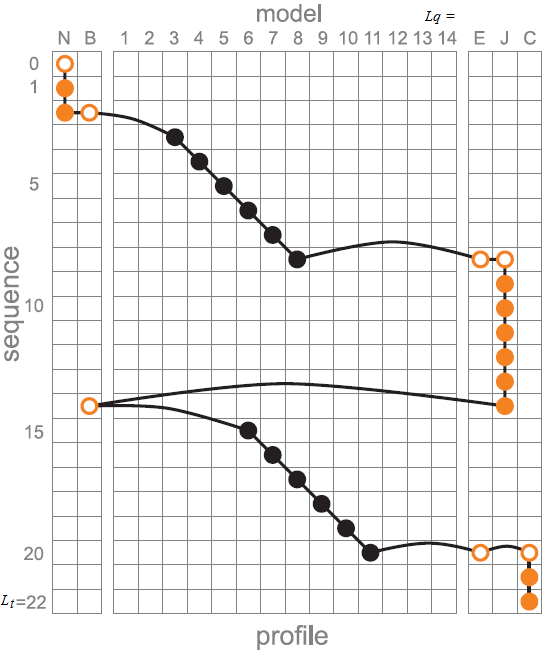
\includegraphics[width=100mm]{Figures/dpMSV.png}
	\caption{\fontfamily{pag}\selectfont \textbf{Example of an MSV path in DP matrix \citep{HMMER3}.} 
An alignment of a MSV profile HMM model (length $L_q = 14$) to a target sequence (length $L_t=22$). A path from top to bottom is through a dynamic programming (DP) matrix. The model identifies two high-scoring ungapped alignment segments, as shown in black dots, indicating residues aligned to profile match states. All other residues are assigned to N, J, and C states in the model, as shown in orange dots. Unfilled dot indicates a ``mute'' non-emitting state or state transition.}
	\label{fig:dpMSV}
\end{figure}

\begin{pseudocode}{MSV}{ }
\label{MSV}
\COMMENT{Initialization}\\
N[0] \GETS 0; \ \  B[0] \GETS tr(N, B)\\
E[0] \GETS C[0] \GETS J[0] \GETS -\infty\\
\COMMENT{for every sequence residue i}\\
\FOR i \GETS 1 \TO L_t \DO
\BEGIN
  N[i] \GETS N[i-1] + tr(N, N)\\
  B[i] \GETS max 
  \begin{cases}
   N[i-1] + tr(N, B)\\
   J[i-1] + tr(J, B)
  \end{cases}\\
  M[i,0] \GETS -\infty\\
  \COMMENT{For every model position j from 1 to $L_q$}\\
  \FOR j \GETS 1 \TO L_q \DO
  \BEGIN
    M[0, j] \GETS -\infty\\
    M[i, j] \GETS e(M_j, S[i]) + max 
    \begin{cases}
     M[i-1, j-1]\\
     B[i-1] + tr(B, M_j)
    \end{cases}\\
  \END\\
  E[i] \GETS max\{M[i,j] + tr(M_j, E)\} \ \  (j \GETS 0 \TO L_q)\\
  J[i] \GETS max 
  \begin{cases}
   J[i-1] + tr(J, J)\\
   E[i-1] + tr(E, J)
  \end{cases}\\
  C[i] \GETS max
  \begin{cases}
   C[i-1] + tr(C, C)\\
   E[i-1] + tr(E, C)
  \end{cases}\\
\END\\
\COMMENT{Termination: }\\
\RETURN {T(S,M) \GETS C[L_t] + tr(C,T)}
\end{pseudocode}

\subsubsection{SIMD vectorized MSV in HMMER3}
\label{SSE2}

Single-Instruction Multiple-Data (SIMD) instruction is able to perform the same operation on multiple pieces of data in parallel. The first widely-deployed desktop SIMD was with Intel's MMX extensions to the x86 architecture in 1996. In 1999, Intel introduced Streaming SIMD Extensions (SSE) in Pentium III series processors. The modern SIMD vector instruction sets use 128-bit vector registers to compute up to 16 simultaneous operations. Due to the huge number of iterations in the Smith-Waterman algorithm calculation, using SIMD instructions to reduce the number of instructions needed to perform one cell calculation has a significant impact on the execution time. Several SIMD vector parallelization methods have been described for accelerating SW dynamic programming. 

In 2000, Rognes and Seeberg presented an implementation of the SW algorithm running on the Intel Pentium processor using the MMX SIMD instructions \citep{SW-SIMD}. They used a query profile parallel to the query sequence for each possible residue. A query profile was pre-calculated in a sequential layout just once before searching database. A six-fold speedup was reported over an optimized non-SIMD implementation. 

In 2007, Farrar presented an efficient vector-parallel approach called striped layout for vectorizing SW algorithm \citep{SW-SSE2}. He designed a striped query profile for SIMD vector computation. He used Intel SSE2 to implement his design. A speedup of 2-8 times was reported over the Rognes and Seeberg SIMD non-stripped implementations.

Inspired by Farrar, in HMMER3\citep{HMMER3}, Sean R. Eddy used a remarkably efficient stripped vector-parallel approach to calculate MSV alignment scores. To maximize parallelism, he implemented MSV as a 16-fold parallel calculation with score values stored as 8-bit byte integers. He used SSE2 instructions on Intel-compatible systems and Altivec/VMX instructions on PowerPC systems.

Figure \ref{fig:strip} shows the stripped pattern. The query profile HMM of length $L_q$ is divided into vectors with equal length $L_v$. The vector length $L_v$ is equal to the number of elements being processed in the 128-bit SIMD register. MSV processes 8-bit byte integer with $L_v$ = 128/8 = 16. In a row-vectorized implementation, the query profile HMM is stored in the vectorized dynamic programming matrix dp. The dp stores $L_q$ cells in $L_Q$ vectors which is numbered as $q = 1...L_Q$, where $L_Q = (L_q+L_v-1)/L_v$. Figure \ref{fig:strip} illustrates $L_q$ cells assigned to $L_Q$ vectors in a non-sequential way. For simple illustration, $L_v = 4, L_q = 14$, and $L_Q = 4$.

\begin{figure}[!htb]
	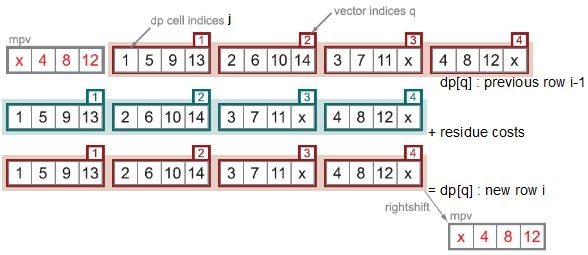
\includegraphics{Figures/msv_vector.jpg}
	\caption{\fontfamily{pag}\selectfont Illustration of striped indexing for SIMD vector calculations\citep{HMMER3}.}
	\label{fig:strip}
\end{figure}

In Smith-Waterman and Viterbi dynamic programming, the calculation of each cell $(i, j)$ in the dp is dependent on previously calculated cells $(i-1, j), (i, j-1)$ and $(i-1, j-1)$. However, in MSV algorithm, the \emph{delete} and \emph{insert} states have been removed and only ungapped diagonals need calculating, so the calculation of each cell $(i, j)$ requires only previous $(i-1, j-1)$. In Figure \ref{fig:strip}, the top red row shows the previous row $i-1$ for the cells $j-1$, which is needed for calculating each new cell $j$ in a new row $i$. 

Striping method can remove the SIMD register data dependencies. As can be seen in the Figure \ref{fig:strip}, with striped indexing, vector $q-1$ contains exactly the four $j-1$ cells needed to calculate the four cells $j$ in a new vector $q$ on a new blue row of the dp matrix. For example, when we calculate cells $j=(2,6,10,14)$ in vector $q=2$, we access the previous row’s vector $q-1=1$ which contains the cells we need in the order we need them, $j-1=(1,5,9,13)$ (the vector above). 

\begin{figure}[!htb]
\centering
	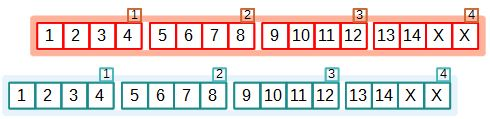
\includegraphics[width=110mm]{Figures/msv_nostrip.jpg}
	\caption{\fontfamily{pag}\selectfont Illustration of linear indexing for SIMD vector calculations.}
	\label{fig:nostrip}
\end{figure}

Instead, if we indexed cells into vectors in the linear order ($j=1,2,3,4$ in vector $q=1$ and so on), as shown in Figure \ref{fig:nostrip}, there is no such correspondence of $(q,q-1)$ with four $(j-1,j)$, and each calculation of a new vector $q$ would require extra expensive operations, such as shifting or rearranging cell values inside the previous row's vectors. By using the striped query access, only one shift operation is needed per row as shown in \ref{fig:strip}. Outside the inner loop(for $q = 1$ to $L_Q$), the last vector on each finished row is right-shifted (mpv, in grey with red cell $j$ indices) and used to initialize the next row calculation.

The pseudo code for the implementation is shown in Algorithm \ref{MSV-SIMD}

\begin{pseudocode}{MSV-SIMD}{ }
\label{MSV-SIMD}
\COMMENT{Initialization}\\
xJ \GETS 0; \ \  dp[q] \GETS vec\_splat(0) \  (q \GETS 0 \TO L_Q-1)\\
xB \GETS base + tr(N, B)\\
xBv \GETS vec\_adds(xB, tr(B, M))\\
\COMMENT{for every sequence residue i}\\
\FOR i \GETS 1 \TO L_t \DO
\BEGIN
  xEv \GETS vec\_splat(0)\\
  mpv \GETS vec\_rightshift(dp[L_Q-1])\\
  \FOR q \GETS 0 \TO L_Q-1 \DO
  \BEGIN
    \COMMENT{temporary  storage of 1 current row value in progress}\\
    tmpv \GETS vec\_max(mpv, xBv)\\
    tmpv \GETS vec\_adds(tmpv, e(M_j, S[i]))\\
    xEv \GETS vec\_max(xEv, tmpv)\\
    mpv \GETS dp[q]\\
    dp[q] \GETS tmpv\\
  \END\\
  xE \GETS vec\_hmax(xEv)\\
  xJ \GETS max 
  \begin{cases}
   xJ\\
   xE + tr(E, J)
  \end{cases}\\
  xB \GETS max 
  \begin{cases}
   base\\
   xJ + tr(J, B)
  \end{cases}\\
\END\\
\COMMENT{Termination: }\\
\RETURN {T(S,M) \GETS xJ + tr(C,T)}
\end{pseudocode}

Five pseudocode vector instructions for operations on 8-bit integers are used in the pseudo code. Either scalars $x$ or vectors v containing 16 8-bit integer elements numbered $v[0]...v[15]$. Each of these operations are either available or easily constructed in Intel SSE2 intrinsics as shown in the following table.

% \begin{minipage}{\textwidth}
% \begin{center}
% \begin{tabular}{|c|c|c|}\hline
% \shortstack{\textbf{Pseudocode} \\ SSE2 code in C} & \textbf{Operation} & \textbf{Definition}\\\hline
% \shortstack{\textbf{v = vec\_splat(x)} \\ v = \_mm\_set1\_epi8(x)} & assignment & $v[z] = x$\\\hline
% \shortstack{\textbf{v = vec\_adds(v1, v2)} \\ v = \_mm\_adds\_epu8(v1, v2)} & saturated addition & $v[z] = min$
% $\begin{cases}
%   2^8-1\\
%   v1[z]+v2[z]
% \end{cases}$\\\hline
% \shortstack{\textbf{v1 = vec\_rightshift(v2)} \\ v1 = \_mm\_slli\_si128(v2, 1)} & right shift & \shortstack{$v1[z] = v2[z-1](z=16...1)$; \\ $v1[0]=0;$}\\\hline
% \shortstack{\textbf{v = vec\_max(v1, v2)} \\ v = \_mm\_max\_epu8(v1, v2)} & max & $v[z] = max(v1[z], v2[z])$\\\hline
% \shortstack{\textbf{x = vec\_hmax(v)} \\ -} & horizontal max & $x = max_zv[z]$\\\hline
% \end{tabular}
% \end{center}
% \end{minipage}


\begin{table}[H]
\centering
\begin{tabular}{|c|c|c|}\hline
\shortstack{\textbf{Pseudocode} \\ SSE2 intrinsic in C} & \textbf{Operation} & \textbf{Definition}\\\hline
\shortstack{\textbf{v = vec\_splat(x)} \\ v = \_mm\_set1\_epi8(x)} & assignment & $v[z] = x$\\\hline
\shortstack{\textbf{v = vec\_adds(v1, v2)} \\ v = \_mm\_adds\_epu8(v1, v2)} & saturated addition & $v[z] = min$
$\begin{cases}
  2^8-1\\
  v1[z]+v2[z]
\end{cases}$\\\hline
\shortstack{\textbf{v1 = vec\_rightshift(v2)} \\ v1 = \_mm\_slli\_si128(v2, 1)} & right shift & \shortstack{$v1[z] = v2[z-1](z=15...1)$; \\ $v1[0]=0;$}\\\hline
\shortstack{\textbf{v = vec\_max(v1, v2)} \\ v = \_mm\_max\_epu8(v1, v2)} & max & $v[z] = max(v1[z], v2[z])$\\\hline
\shortstack{\textbf{x = vec\_hmax(v)} \\ -} & horizontal max & $x = max(v[z]),z=0...15$\\\hline
\end{tabular}
\caption{\fontfamily{pag}\selectfont\textbf{SSE2 intrinsics for pseudocode in Algorithm \ref{MSV-SIMD}} The first column is pseudocode and its corresponding SSE2 intrinsic in C language. Because x86 and x86-64 use little endian, \textbf{vec\_rightshift()} means using a left bit shift intrinsic \textbf{\_mm\_slli\_si128()} to do right shift. No SSE2 intrinsic is corresponding to \textbf{vec\_hmax()}. Shuffle intrinsic \textbf{\_mm\_shuffle\_epi32} and \textbf{\_mm\_max\_epu8} can be combined to implement \textbf{vec\_hmax()}.\label{tab.SSE2}}
\end{table}


%----------------------------------------------------------------------------------------

\section{CUDA accelerated sequence alignment}
\label{CUDASeqAlign}

In November 2006, NVIDIA\textregistered introduced CUDA\texttrademark (Compute Unified Device Architecture), a general purpose parallel computing platform and programming model that enables users to write scalable multi-threaded programs in NVIDIA GPUs. Nowadays there exist alternatives to CUDA, such as OpenCL \citep{OpenCL}, Microsoft Compute Shader\citep{Shader}. These are mostly similar, but as CUDA is the most widely used and more mature, this thesis will focus on that.

This section firstly overviews CUDA programming model, then reviews recent studies on accelerating Smith-waterman algorithm and HMM-based algorithms on CUDA-enabled GPU.

\subsection{Overview of CUDA programming model}
\subsubsection{Streaming Multiprocessors}
A GPU consists of one or more SMs(Streaming Multiprocessors). Quadro K4000 used in our research has 4 SMs. Each SM contains the following specific features \citep{CUDAHand}:

\begin{itemize}
 \item Execution units to perform integer and single- or double-precision floating-point arithmetic, Special function units (SFUs) to compute single-precision floating-point transcendental functions
 \item Thousands of registers to be partitioned among threads
 \item Shared memory for fast data interchange between threads
 \item Several caches, including constant cache, texture cache and L1 cache
 \item A warp scheduler to coordinate instruction dispatch to the execution units
\end{itemize}

The SM has been evolving rapidly since the introduction of the first CUDA-enabled GPU device in 2006, with three major Compute Capability 1.x, 2.x, and 3.x, corresponding to Tesla-class, Fermi-class, and Kepler-class hardware respectively. Table \ref{tab.sm} summarizes the features introduced in each generation of the SM hardware \citep{CUDAHand}.

\begin{table}[H]
\begin{tabular}[t]{|c|c|}\hline
\shortstack{\textbf{Compute}\\ \textbf{Capability} } & \textbf{Features introduced} \\\hline
SM 1.x & \shortstack[l]{Global memory atomics; mapped pinned memory; debuggable;\\ atomic operations on shared memory; Double precision} \\\hline
{SM 2.x} & \shortstack[l]{64-bit addressing; L1 and L2 cache; concurrent kernel execution;\\ global atomic add for single-precision floating-point values;\\ Function calls and indirect calls in kernels} \\\hline
SM 3.x & \shortstack[l]{SIMD Video Instructions; Increase maximum grid size; warp shuffle;\\ Bindless textures (``texture objects''); read global memory via texture;\\ faster global atomics; 64-bit atomic min, max, AND, OR, and XOR;\\ dynamic parallelism} \\\hline
\end{tabular}
\caption{\fontfamily{pag}\selectfont Features per Compute Capability\label{tab.sm}}
\end{table}

\subsubsection{CUDA thread hierarchy}
The execution of a typical CUDA program is illustrated in Figure \ref{fig:exeCUDA} The CPU host invokes a GPU kernel in-line with the triple angle-bracket $<<<$  $>>>$ syntax from CUDA C/C++ extension code. The kernel is executed N times in parallel by N different CUDA threads. All the threads that are generated by a kernel during an invocation are collectively called a \emph{grid}. Figure \ref{fig:exeCUDA} shows the execution of two grids of threads.

\begin{figure}[!htb]
	\centering
	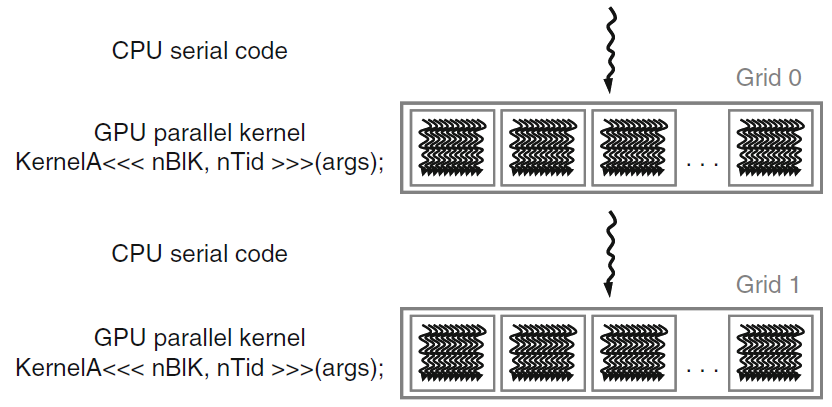
\includegraphics[totalheight=0.2\textheight]{Figures/exeCUDA.png}
	\caption{\fontfamily{pag}\selectfont Execution of a CUDA program\citep{Kirk}.}
	\label{fig:exeCUDA}
\end{figure}

Threads in a grid are organized into a two-level hierarchy, as illustrated in Figure \ref{fig:grid}. At the top level, each grid consists of one or more thread blocks. All blocks in a grid have the same number of threads and are organized into a one, two, or three-dimensional \emph{grid} of thread blocks.

\begin{figure}[!htb]
	\centering
	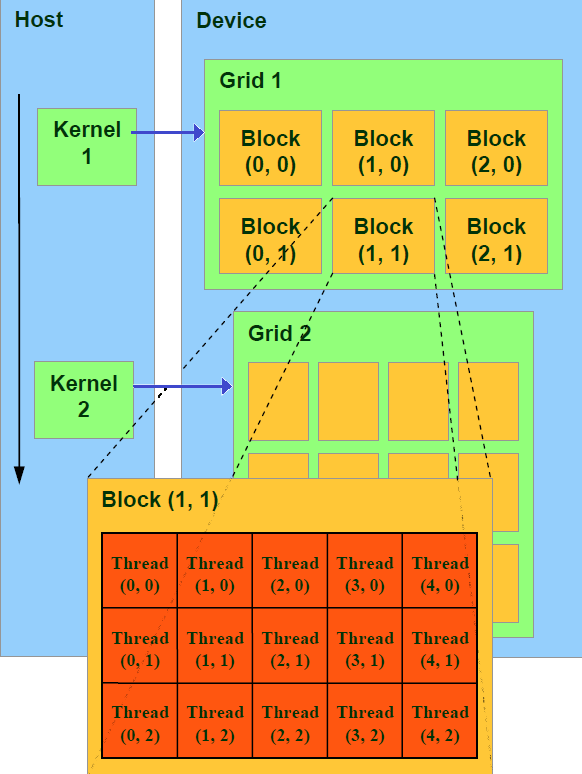
\includegraphics[totalheight=0.4\textheight]{Figures/gridBlock.png}
	\caption{\fontfamily{pag}\selectfont CUDA thread organization\citep{Zeller}.}
	\label{fig:grid}
\end{figure}

Each block can be identified by an index accessible within the kernel through the built-in \emph{blockIdx} variable. The dimension of the thread block is accessible within the kernel through the built-in \emph{blockDim} variable.

The threads in a block are executed by the same multiprocessor within a GPU. They can cooperate by sharing data through some shared memory and by synchronizing their execution to coordinate memory accesses. Each block can be scheduled on any of the available multiprocessors, in any order, concurrently or sequentially, so that a compiled CUDA program can execute on any number of multiprocessors. On the hardware level, a block's threads are executed in parallel as \emph{warps} which name originate from \emph{weaving loom}. A warp consists of 32 threads.

\subsubsection{CUDA memory hierarchy}
\label{cudaMemH}
Besides the threading model, another thing that makes CUDA programming different from a general purpose CPU is its memory spaces, including registers, local, shared, global, constant and texture, as shown in Figure \ref{fig:cudaMem}

\begin{figure}[!htb]
	\centering
	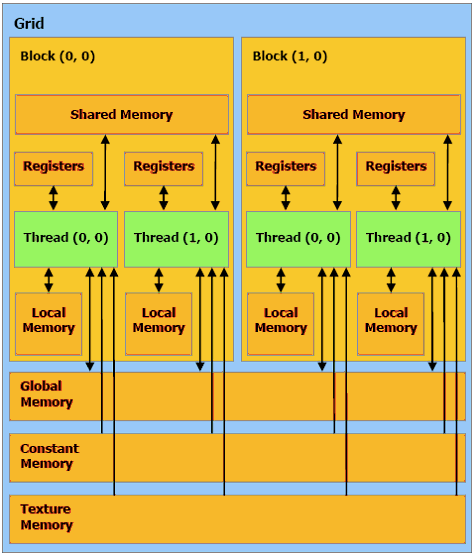
\includegraphics[totalheight=0.4\textheight]{Figures/cudaMem.png}
	\caption{\fontfamily{pag}\selectfont CUDA memory organization\citep{Zeller}.}
	\label{fig:cudaMem}
\end{figure}

CUDA memory spaces have different characteristics that reflect their distinct usages in CUDA applications as summarized in Table \ref{tab.mem} \citep{CUDABest}.

\begin{table}[H]
\centering
\begin{tabular}{|c|c|c|c|c|c|c|}\hline
\textbf{Memory} & \textbf{Location} & \textbf{Cached} & \textbf{Access} & \textbf{Scope} & \textbf{Speed} & \textbf{Lifetime} \\\hline
Register & On chip & n/a & R/W & 1 Thread & 1 & Thread \\\hline
Local & Off chip & \dag & R/W & 1 Thread & $\sim 2 - 16$ & Thread \\\hline
Shared & On chip & n/a & R/W & \shortstack{All threads\\ in block} & $\sim 2 - 16$ & Block \\\hline
Global & Off chip & \dag & R/W & \shortstack{All threads\\ + host} & 200+ & Host allocation \\\hline
Constant & Off chip & Yes & R & \shortstack{All threads\\ + host} & $2 - 200$ & Host allocation \\\hline
Texture & Off chip & Yes & R & \shortstack{All threads\\ + host} & $2 - 200$ & Host allocation \\\hline
\end{tabular}
\caption{\fontfamily{pag}\selectfont \textbf{Salient Features of GPU Device Memory.} \textbf{Speed} column is the relative speed in number of instructions. {\dag} means it is cached only on devices of above compute capability 2.x. \label{tab.mem}}
\end{table}

\subsubsection{CUDA tools}
\label{cudaTools}

The NVIDIA CUDA Toolkit provides a comprehensive development environment for C/C++ developers building GPU-accelerated applications. The CUDA Toolkit is available at \url{https://developer.nvidia.com/cuda-toolkit}, including a compiler \emph{nvcc} for NVIDIA GPUs, math libraries, and tools for debugging and optimizing the performance of CUDA applications.

\textbf{Nsight Eclipse Edition}\\
NVIDIA Nsight Eclipse Edition is a full-featured IDE powered by the Eclipse platform that provides an all-in-one integrated programming environment for editing, building, debugging and profiling CUDA C/C++ applications. Nsight Eclipse Edition supports a rich set of commercial and free plugins.
Nsight Eclipse Edition ships as part of the CUDA Toolkit Installer for Linux and Mac at \url{https://developer.nvidia.com/nsight-eclipse-edition}.

\textbf{NVIDIA Nsight Visual Studio Edition}\\
NVIDIA provides Nsight Visual Studio Edition to integrate seamlessly into Microsoft Visual Studio environment at\\ \url{https://developer.nvidia.com/nvidia-nsight-visual-studio-edition}. It can\\ build, debug, profile and trace heterogeneous compute and graphics applications using CUDA C/C++, OpenCL \citep{OpenCL}, DirectCompute \citep{Shader}, Direct3D, and OpenGL.

\textbf{Profiling tools}\\
 NVIDIA® provides profiling tools to help execute the kernels in question under the watchful gaze, which are publicly available as a separate download on the CUDA Zone website \citep{CUDAzone}.
 
% \begin{table}[H]
% \centering
% \begin{tabular}{|c|c|c|c|}\hline
% \shortstack{\textbf{Tools Name}} & \shortstack{\textbf{Command}} & \shortstack{\textbf{OS}} & \shortstack{\textbf{User interface}}\\\hline
% nvprof & nvprof & \shortstack{Linux, Mac OS X\\ and Windows} & command-line\\\hline
% Visual Profiler & nvvp & \shortstack{Linux, Mac OS X\\ and Windows} & graphical \\\hline
% Nsight™ Ecipse Edition & nsight & Linux and Mac OSX & graphical\\\hline
% \shortstack{NVIDIA® Nsight™ \\ Visual Studio Edition} & -\tablefootnote[12]{Integrated into Microsoft Visual Studio} & Windows & graphical\\\hline
% Parallel Nsight™ & - & Windows & graphical\\\hline
% \end{tabular}
% \caption{CUDA profiling tools\label{tab.prof}}
% \end{table}

\begin{table}[H]
\centering
\begin{tabular}{|c|c|c|c|}\hline
\shortstack{\textbf{Tools Name}} & \shortstack{\textbf{OS}} & \shortstack{\textbf{User interface}}\\\hline
nvprof & \shortstack{Linux, Mac OS X\\ and Windows} & command-line\\\hline
Visual Profiler & \shortstack{Linux, Mac OS X\\ and Windows} & graphical \\\hline
Nsight™ Ecipse Edition & Linux and Mac OSX & graphical\\\hline
\shortstack{NVIDIA® Nsight™ \\ Visual Studio Edition} & Windows & graphical\\\hline
Parallel Nsight™ & Windows & graphical\\\hline
\end{tabular}
\caption{\fontfamily{pag}\selectfont {CUDA profiling tools}\label{tab.prof}}
\end{table}

\textbf{Nvidia-SMI}\\
The NVIDIA System Management Interface (nvidia-smi) is a command line utility that helps managing and monitoring GPU devices. It ships with NVIDIA GPU display drivers on Linux and Windows. This utility allows administrators to query GPU device state and modify GPU device state. It can also report control aspects of GPU execution, such as whether ECC is enabled and how many CUDA contexts can be created on a given GPU.

% http://docs.nvidia.com/cuda/profiler-users-guide/#axzz32CP5hrTb
%----------------------------------------------------------------------------------------

\subsection{CUDA accelerated Smith-Waterman}
The Smith-Waterman algorithm exploits dynamic programming for sequence alignment, which is also the characteristic of HMM-based algorithms. In this section, we review the techniques used in parallelizing Smith-Waterman on a CUDA-enabled GPU and these techniques will be evaluated for accelerating MSV algorithm in Chapter \ref{CUDAHMMER3}.

\subsubsection*{Parallelism strategy applied}
\textbf{1) Task-based parallelism}

As explained in Section \ref{impl}, parallel computing has two types of parallelism: task-based and data-based parallelism. SW algorithm is used for finding similarity among protein sequence database with dynamic programming. The application is particularly well-suited for many-core architectures due to the parallel nature of sequence database searches. 

Liu et al. have been studying accelerating Smith-Waterman sequence database searches for CUDA-enabled GPU since 2009. Here are their 3 articles from 2009 to 2013: \citep{SW++}, \citep{SW++2} and \citep{SW++3}. They present many approaches for optimization. They use task-based parallelism to process each target sequence independently with a single GPU thread. Task-based parallelism removes the need for inter-thread communications or, even worse, inter-multiprocessor communications. This also simplifies implementation and testing. 

Due to these reasons, task-based parallelism has been taken by most of studies and more efforts are put on optimizing CUDA kernel execution. Among 8 articles reviewed here, 7 articles apply this approach. Beside 3 articles of Liu et al., other 4 article are \citep{Manavski}, \citep{Akoglu}, \citep{Ligowski} and \citep{Kentie}.

In \citep{SW++3}, Liu et al. not only distribute tasks to many threads in GPU kernel, but also balance the workload between CPU and GPU. Their distribution policy calculates a rate $R$ of the number of residues from the database assigned to GPUs, with a formular as

\begin{equation*}
  R = \frac{N_Gf_G}{N_Gf_G + N_Cf_C / C}
\end{equation*}

where $f_C$ and $f_G$ are the core frequencies of CPUs and GPUs, $N_C$ and $N_G$ are the number of CPU cores and the number of GPU SMs, and C is a constant derived from empirical evaluations.

They find the sequence length deviation generally causes execution imbalance between threads, which in return can not fully utilize GPU compute power. Considering this, they design two CUDA kernels based on two parallelization approaches: static scheduling and dynamic scheduling. These two kernels are launched based on the sequence length deviation of the database. 

Since each thread has its own buffers in global memory, the static scheduling launches all thread blocks onto the GPU at the same time. When a thread block finishes its current computation, this thread block will use the dynamic scheduling to obtain an unprocessed profile block. They use the atomic addition function \emph{atomicAdd}() to increment the index of global profile blocks.

\citep{Manavski} also distributes some tasks to CPU. In GPU, they only launch 450 thread-blocks at a time on a grid. For a database with sequences more than 450, several kernel launches are necessary and this will create additional latency. And since they run 64 threads per block. So, they can only process 450 * 64 = 28,800 alignments per kernel launch. CUDA limits the number of blocks in a grid to 65,535 blocks in a single dimension, which is far above the threshold they are using. This results in low GPU kernel thread occupancy.

Considering Manavski's implementation limitation in thread occupancy, \citep{Akoglu} sets thread block size by the total number of sequences located in the database so that they can to do all alignments with a single kernel launch.

In order to achieve high efficiency for task-based parallelism, the run time of all threads in a thread block should be roughly identical. Therefore many studies often sorted sequences databases by length of sequences. Thus, for two adjacent threads in a thread warp, the difference value between the lengths of the associated sequences is minimized, thereby balancing a similar workload over threads in a warp.

\citep{Manavski}, \citep{Akoglu}, \citep{SW++}, \citep{SW++2} and \citep{SW++3} presorted database in ascending order.

\citep{Ligowski} presorts database in descending order and organizes data in blocks consisting of 256 sequences, since each kernel has 16 blocks, and a single block consists of 256 threads. The choice of 4096 threads per kernel is dictated partially by limitations of architecture and partially by optimization of performance. There are 16 multiprocessors in each core, each executes a single block of threads. The number of 256 threads per block is limited by the number of registers (8192 per multiprocessor). The SW main routine needs 29 registers, and therefore the highest multiply of 64 that can be concurrently executed is 256.
They process the alignment matrix horizontally. The main loop for calculating the matrix is executed for a band of 12 cells columns. Slow global memory is accessed only at the initialization and termination of the loop. Fast shared memory and registers are used for all operations within the loop. The width of the band is limited by availability of shared memory.

\citep{Kentie} implements a \emph{dbconv} tool to presort database also in descending order and converted into a special format. The \emph{dbconv} writes the sorted sequences to file in an interlaced fashion: the database is split up into half-warp sized blocks of 16 sequences. The sequences of a block are written in an alternating fashion: one 8-bit symbol of the first sequence is written, then one of the second one, etc. In this way, the first character of all 16 sequences is written, then the second character, etc. All sequences in a rectangular block are padded to the length of the block's longest sequence with blank symbols. By this way, all of a half-warp's threads will load database symbols from neighboring addresses so as to access the global memory in coalesced way.

\textbf{2) Data-based parallelism}

In data-based parallelism, each task is assigned to one or many thread block(s) and all threads in the thread block(s) cooperate to perform the task in parallel.

The main target of \citep{Saeed} is to solve a single but very large Smith-Waterman problem for sequences with very long lengths. Their calculation work along anti-diagonals of the alignment matrix. Each diagonal item can be calculated independently of the others. Block diagonal algorithms are also possible as long as each block is processed serially.

They formulate parallel version of the Smith-Waterman algorithm so that the calculations can be performed in parallel one row (or column) of similarity matrix at a time. Row (or column) calculations allow the GPU global memory accesses to be consecutive and therefore high memory throughput is achieved.

They exploit approach of parallelizing multiple GPUs with using MPI (Message Passing Interface) parallel technique over 100 Mb Ethernet to extend work to multiple GPUs. To use N GPUs, the Smith-Waterman alignment matrix is decomposed into N large, and slightly overlapping blocks. 

\citep{SW++} investigate the two parallelism approaches for parallelizing the sequence database searches using CUDA. They find task-based parallelism can achieve better performance although it needs more device memory than data-based. 
For task-based parallelism, they sort target sequences and store in an array row by row from the top-left corner to the bottom-right corner, where all symbols of a sequence are restricted to be stored in the same row from left to right. Using these arrangement patterns for the two parallelism strategies, access to the target sequences is coalesced for all threads in a half-warp. 

To maximize performance and to reduce the bandwidth demand of global memory, they also apply a cell block division method for the task-based parallelism, where the alignment matrix is divided into cell blocks of equal size.

They apply data-based parallelism to support longest query/target sequences. Each task is assigned to one thread block and all threads in the thread block cooperate to perform the task in parallel, exploiting the parallel characteristics of cells in the minor diagonals of similarity matrix. 

\subsubsection*{Device memory access pattern}
As described in Section \ref{cudaMemH}, CUDA memory hierarchy includes registers, local, shared, global, constant and texture, as shown in Figure \ref{fig:cudaMem}. Memory throughput generally dominates program performance both in the CPU and GPU domains. Here is the reviewing of how these studies applied different device memory access pattern to optimize their implementations.

\citep{SW++} sorts target sequences and arranges in an array like a multi-layer bookcase to store into global memory, so that the reading of the database across multiple threads could be coalesced. Writes to global memory are first batched in shared memory for better coalescing. Due to a reduction in the global memory accesses, they propose a cell block division method for the task-based parallelism, where the alignment matrix is divided into cell blocks of equal size.
And they utilize the texture memory on the sorted array of target sequences in order to achieve maximum performance on coalesced access patterns. They use a hash table to index the location coordinate in the array and the length of each sequence, which can provide fast access to any sequence.

They also exploit constant memory to store the gap penalties, scoring matrix and the query sequence. They load the scoring matrix into shared memory, as the performance of constant memory degrades linearly when threads frequently need to access multiple different addresses in the scoring matrix. They also use the CUDA built-int integer functions max(x, y) and min(x, y) to improve performance further.

\citep{Kentie} reduces global memory access by making temporary values interleaved and reads/writes score and Ix temporary values in one access.
And Kentie exploits constant memory and shared memory for substitution matrix. Constant memory is fast, but only if all threads read the same address. This is not suited to the substitution matrix. And shared memory also has several disadvantages for the matrix. Finally, he finds texture memory has the ability to fetch four values at a time and is well suitable for random access. He gains a total speedup of 25\% after switching from shared to texture memory.
He also stores gap penalties in constant memory. 

\citep{Akoglu} stores database sequences in global memory. The cell calculation blocks are used to store temporary calculation values needed for data dependencies for each column and are also stored in global memory. They use the substitution matrix instead of the query profile to save memory size. In order to index the row and column of the matrix in extremely efficient way, they design a simple function for accessing the matrix, which is as follows:

$S_{i,j} = (ascii(S_1)-65, ascii(S_2)-65)$

$S_1$ is a residue from the query sequence and $S_2$ is a residue from one of the Database sequences.
They map query sequence as well as the substitution matrix to the constant memory to make access to these values easy.
They track the highest SW score by a single register in the kernel for each thread, and update on each pass of the inner loop. Then the score is written to the global memory, after the alignment is finished.

Among the 7 articles reviewed here, \citep{Manavski} is the first to study accelerating SW on CUDA-enabled GPU in 2007. They present the query profile as a query-specific substitution matrix computed only once for the entire database. They exploit the cache of texture memory to store query profiles. In this way they replace random accesses to the substitution matrix with sequential ones to the query profile. 

\citep{SW++2} utilizes texture memory to store query profiles. They use shared memory to store the 4 residues of target sequence. 

\citep{SW++3} stores both the query profile and its variant in texture memory. They gain more performance from the query profile variant for short queries,  because it can reduce the number of texture fetches by half. However, for longer queries, a query profile becomes superior due to its much smaller memory footprint and less texture cache miss. They apply a query length threshold Q to decide whether to use the query profile or the variant.

\citep{Ligowski} reduces global memory access only at the loop initialization and for writing the results at the exit. They performed all operations within the loop in fast shared memory and registers.

\subsubsection*{Vector programming model}
Vector programming model plays important role in operations of array or matrix. On one side, it can reduce greatly the frequency of memory access; on the other side, it can utilize the built-in SIMD vector instructions for parallel computing both on CPU and GPU.

\citep{Manavski} packs the query profile in texture memory, storing 4 successive values into the 4-byte of a single unsigned integer. To compute a column of alignment matrix, all the H and E values are needed from the previous one. They place them in the two local memory buffer of the thread: one for the previous values and another for the newly computed ones. At the end of each column they swap them. Since local memory is not cached, they use specific access pattern to read 4 H and 4 E values from local memory at a time, which can fully take advantage of the 128 bits memory bandwidth. Thus, each thread can gather all the data needed to compute 4 cells of the alignment matrix with only two read instructions: one from the local buffer and another from the texture.

Manavski pre-computes a query profile parallel to the query sequence for each possible residue and achieves dynamic load balancing between multiple GPUs according to their computational power at run time.

\citep{Akoglu} calculates the Smith-Waterman score from the query sequence and database sequences by means of columns, 4 cells at a time for the residue of database sequence aligned with an 8 residue query sequence. The updated values of cells are placed in a temporary location in the global memory. This cell calculation block is updated each time a new column is computed, and is utilized for dependency purposes in computing columns on each pass.

\citep{SW++2} designs a striped query profile for SIMD vector computation and uses a packed data format to store into the CUDA built-in \emph{uchar4} vector data type, instead of the \emph{char} scalar data type. In this way, 4 substitution scores can be accessed with only one texture fetch, thus greatly improving texture memory throughput.

Like the query profile, they also construct each target sequence with a packed data format, where 4 successive residues of each target sequence are packed together and placed in \emph{uchar4}. In this case, they utilize shared memory to store the 4 residues loaded by one texture fetch for the use of the inner loop, when using the cell block division method.

Since CUDA lacks support for saturation addition and subtraction, they use maximum and minimum operation to artificially implement them. The CUDA built-in integer functions max(x, y) and min(x, y) are utilized to avoid divergence. They implement shift operation on vector using shared memory, where all threads comprising a virtualized vector write their original values to a share memory buffer and then read their resulting values from the buffer as per the number
of shift elements. 

They divide a query sequence into a series of non-overlapping, consecutive small partitions with a specified partition length, and then align the query sequence to a subject sequence partition by partition. They port the SIMD CPU algorithm \citep{SW-SSE2} to the GPU, viewing collections of processing elements as part of a single vector.

\citep{Kentie} applies vector data structure to load 4 query characters at a time and processes 8 database characters at a time. He loads query profile values for the 4 current query characters and passes them to the Smith-Waterman function. The 4 query symbols and loaded query profile values are aligned with each loaded database symbol.

And he simplifies substitution matrix lookup by using numeric values instead of letters for sequence symbols.

\citep{SW++3} designs a query profile variant data structure and packs the 4 consecutive elements of variant data into the built-in \emph{short4} vector type. In this way, although the variant data need more memory space compared to the query profile,  they can reduce the number of texture fetches for the variant by half. On the other side, using the variant can save 6 bitwise operations for generating a substitution score vector.
They also utilize the built-in \emph{uint4} vector data type to store each sequence profile for quad-lane SIMD computing on GPUs. 

They use CUDA SIMD Video Instructions in GPU computing and use Intel SSE2 intrinsic in CPU computing. For CPU SIMD computation, their approach is based on the open-source SWIPE \citep{Rognes}. They compute the SW algorithm by splitting an SSE vector to 16 lanes with 8-bit lane width. Then they re-compute all alignments, whose scores have overflow potential, using 8-lane SSE vectors with 16-bit lane width.

%----------------------------------------------------------------------------------------

\subsection{CUDA accelerated HMMER}
HMMER includes a MPI (Message Passing Interface) implementation of the searching algorithms, which uses conventional CPU clusters for parallel computing. ClawHMMer \citep{ClawHMMER} is the first GPU-enabled \emph{hmmsearch} implementation. Their implementation is based on the BrookGPU stream programming language, not CUDA programming model. Since ClawHMMer, there has been several researches on accelerating HMMER for CUDA-enabled GPU. The following is the summary of techniques applied by 5 research work.

\subsubsection*{Parallelism strategy applied}
As explained in Section \ref{impl}, parallel computing has two types of parallelism: task-based and data-based parallelism. SW algorithm is used for finding similarity among protein sequence database with dynamic programming method. The application is particularly well-suited for many-core architectures due to the parallel nature of sequence database searches. Among 5 articles reviewed here, 3 articles, i.e. \citep{GPUHMM}, \citep{Quirem} and \citep{Ahmed} used task-based parallelism to process each target sequence independently with a single GPU thread. Task-based parallelism removes the need for inter-thread communications or, even worse, inter-multiprocessor communications. This also simplifies implementation and testing. This approach was taken by most of studies and more efforts were put on optimizing CUDA kernel execution.

In \citep{GPUHMM}, Walters et al. port Viterbi function to CUDA-enabled GPU with a variety of optimization approaches. Their implementation operate the GPU kernel on multiple sequences simultaneously, with each thread operating on an independent sequence. They found the number of threads that can be executed in parallel will be limited by two factors: one is GPU memory will limit the number of sequences that can be placed, and another is the number of registers used by each thread will limit the number of threads that can execute in parallel. And registers are the most important resource in their implementation.

They split the inner loop for computing the dynamic programming matrix into three independent small loops. This approach makes fewer registers be required, resulting in higher GPU utilization. Further, splitting the loop leads an easy mechanism to exploit loop unrolling, which is a classic loop optimization strategy designed to reduce the overhead of inefficient looping. The idea is to replicate the loop�s inner contents such that the percentage of useful instruction to loop extra bound instruction increases. In their experiment, the performance improvement reaches 80\%.

In order to achieve high efficiency for task-based parallelism, the run time of all threads in a thread block should be roughly identical. Therefore many studies often sorted sequences databases by length of sequences. Thus, for two adjacent threads in a thread warp, the difference value between the lengths of the associated sequences is minimized, thereby balancing a similar workload over threads in a warp. Walters et al. presort target sequences database in ascending order. This approach is both effective and quite straightforward way of optimization and they gain a nearly 7x performance improvement over the unsorted database without changing the CUDA kernel in any way.

Walters et al. distribute some tasks to CPU, creating two CPU threads for reading database and post-processing the database hits.

For data-based parallelism, based on the \emph{wave-front} method \citep{Aji}, Du et al. apply a new tile-based mechanism to accelerate the Viterbi algorithm on a single GPU in \citep{Du}. The \emph{wave-front} method compute the cells along anti-diagonal of the dynamic matrix in parallel, which is similar to a frontier of a wave to fill a matrix, where each cell's value in the matrix is computed based on the values of the left, upper, and upper-left cells.

They apply streaming method to process very long sequences. In CUDA, a stream is a set of instructions that execute in order and different streams may execute their instructions asynchronously. This feature enables the execution be overlapped with each other between the host and GPU device.

Since the streaming Viterbi algorithm requires additional storage and communication bandwidth, they design the new tile-based method to simplify the computational model and also handles very long sequences with less memory transfer. The tile-based method handles very long sequence as follows: the large matrix is divided into tiles to ensure that each tile fits in the GPU�s memory as a whole and then compute the tiles in parallel.

Unlike the tiling machanism in \citep{Aji}, which has data dependencies among each tile, they present the \emph{homological segments} concept into their tile-based mechanism to eliminate the data dependency among different tiles. They apply the k-mer based algorithm to find all homological segments. Then the homological segments are used to divide the full dynamic programming matrix into small tiles.

\citep{Ganesan} parallelizes Viterbi algorithm to accelerate hmmsearch. They present a hybrid parallelization strategy by combining task-based and data-based parallelism. They extend the existing task parallelism upon which data parallelism is built. They reassign the computation of a single sequence across multiple threads to implement the data parallelism. In order to accelerate the computation of the dynamic programming matrix rows, they partition each row into equal sized intervals of contiguous cells and calculate the dependencies between the partitions identically and independently in a data parallel setting.

They process the parallel computation of the rows in three phases as follows:

\begin{itemize}
 \item In Phase 1, they use independent threads to compute the relationship between the beginning and end of each partition, which enables the fast computation of boundary elements between the partitions.
 \item In Phase 2, by applying the functions relating the boundary elements from Phase 1, they compute the numeric values for each of the boundary elements. This phase executes consecutively, with N partitions requiring N steps.
 \item In Phase 3, by using the updated numerical values for each of the boundary elements, each partition independently computes the numeric values for all of the elements within the partition in the data parallelism setting.
\end{itemize}

Phase 1 is the critical phase that construct data parallelism by building the relationship among the different partitions. Phases 2 and 3 are computation phases for the boundary and internal elements of partitions.

They implement the partitioning scheme with storing index data of model positions at regular intervals consecutively to achieve coalesced global memory access. They benchmark the implementation on Tesla C1060, showing a speed-up of 5x-8x compared to \citep{GPUHMM} using unsorted database.

\citep{Ahmed} uses Intel� VTune Analyzer \citep{Intel} to investigate performance hotspot functions in HMMER3. Based on hotspot analysis, they study CUDA acceleration for three individual algorithm: Forward, Backward and Viterbi algorithms. And they found data transfer overhead between heterogeneous processors could be a performance bottleneck.

Based on their experiments, they show that Forward, Backward and Viterbi function take 37\%, 31\% and 20\% respectively for the percentage of the total CPU clock. They tested their CUDA implementation of these three functions. Their results show that about 2.27x, 1.58x and 1.50x speedup over the original CPU-only implementation for Forward, Backward and Viterbi function respectively. And they analyze the reason is coming from hotspot analysis. Since Forward function has highest clock time among the three function, it is the most dominant module and CUDA implementation of Forward shows large impact on speedup. Backward is the second one and Viterbi shows least speedup according to hotspot analysis based partial acceleration. They also combine the three modules and show about 2.10x speedup over the original CPU-only implementation.

However, they did not present how they exactly implement their CUDA programs for the three functions and how they accelerate their programs in \citep{Ahmed}

\subsubsection*{Device memory access pattern}
As described in Section \ref{cudaMemH}, CUDA memory hierarchy includes registers, local, shared, global, constant and texture, as shown in Figure \ref{fig:cudaMem}. Memory throughput generally dominates program performance both in the CPU and GPU domains. Here is the reviewing of how these studies applied different device memory access pattern to optimize their implementations.

\citep{GPUHMM} found the most effective optimization for Viterbi algorithm is to optimize CUDA memory layout and usage patterns within the implementation. 

Since Viterbi algorithm requires only the current and previous rows of the dynamic programming matrices, they reduce the memory requirements of the Viterbi scoring calculation from $3 * M * L + 5 * L$ to $6 * M$ integer array elements, where $M$ and $L$ are the length of the sequence and HMM, respectively.

They utilize high speed texture memory to store the target sequence batch. Because the sequence data are static and read-only through computing. They note that global memory coalesced access can significantly improve hmmsearch overall speedup. Their benchmark results show that this approach contributes an improvement of more than 9x for larger HMMs.

They use constant memory and texture memory to store the query profile HMM depending on its size. They place the normal size HMM in constant memory. In cases where the very large HMM exceeds the capacity of constant memory, they switch over to texture memory for the remaining portion of the HMM after exploiting the full constant memory. They utilize shared memory to temporarily store the index into each thread�s digitized sequence.

\citep{Du} reorganizes the computational kernel of the Viterbi algorithm, and divides the basic computing unit into two parts: independent and dependent parts. All of the independent parts are executed with a parallel and balanced load in an optimized coalesced global memory access manner, which significantly improves the Viterbi algorithm�s performance on GPU. 

They implement the \emph{wave-front} pattern using the data skewing strategy. This makes cells in the same parallelizing group be adjacent to each other. In this way, because data accessed by neighbor threads are organized adjacent to each other, threads could access memory in a more efficient manner.

\citep{Quirem} implements Viterbi algorithm being performed on Tesla C1060.

They utilize pinned memory to reduce the latency induced by transferring memory from device to host and back. And they test two different versions of the memory allocation mechanism: one is pageable memory allocation with the standard \emph{malloc} function, another is pinned memory with the \emph{cudaHostAlloc} function. Pinned memory is host memory that can not be paged (swapped) out to disk by the virtual memory management of the OS, and thus reduces the latency induced by transferring memory from device to host and back. Based on their experiments, utilizing pinned memory, the execution of the kernels spends more GPU time relative to the less memory transfer time. Kernel execution time is basically the same for both pageable and pinned memory, because the two versions only relate to the speed of the memory transfer. In their experiments, the performance of pinned memory is improved roughly 20\% over that of pinned memory.

Their implementation gains 10x-15x speedup over the original implementation of the Viterbi function according to the number of queries. They tested up to 16,384 queries because of the limitations of the Tesla C1060 and the speedup increased exponentially as the number of launched threads i.e. number of queries doubled. 
